\begin{figure}
    \centering
    \setlength{\resLen}{2.8in}
    \addtolength{\tabcolsep}{-3pt}
    \small
    \begin{tabular}{cc}
        \begin{overpic}[height=\resLen]{pfunc/color2.png}
            \put(2, 60){Ours}
            \put(2, 1){Single-particle}
        \end{overpic}
        &
        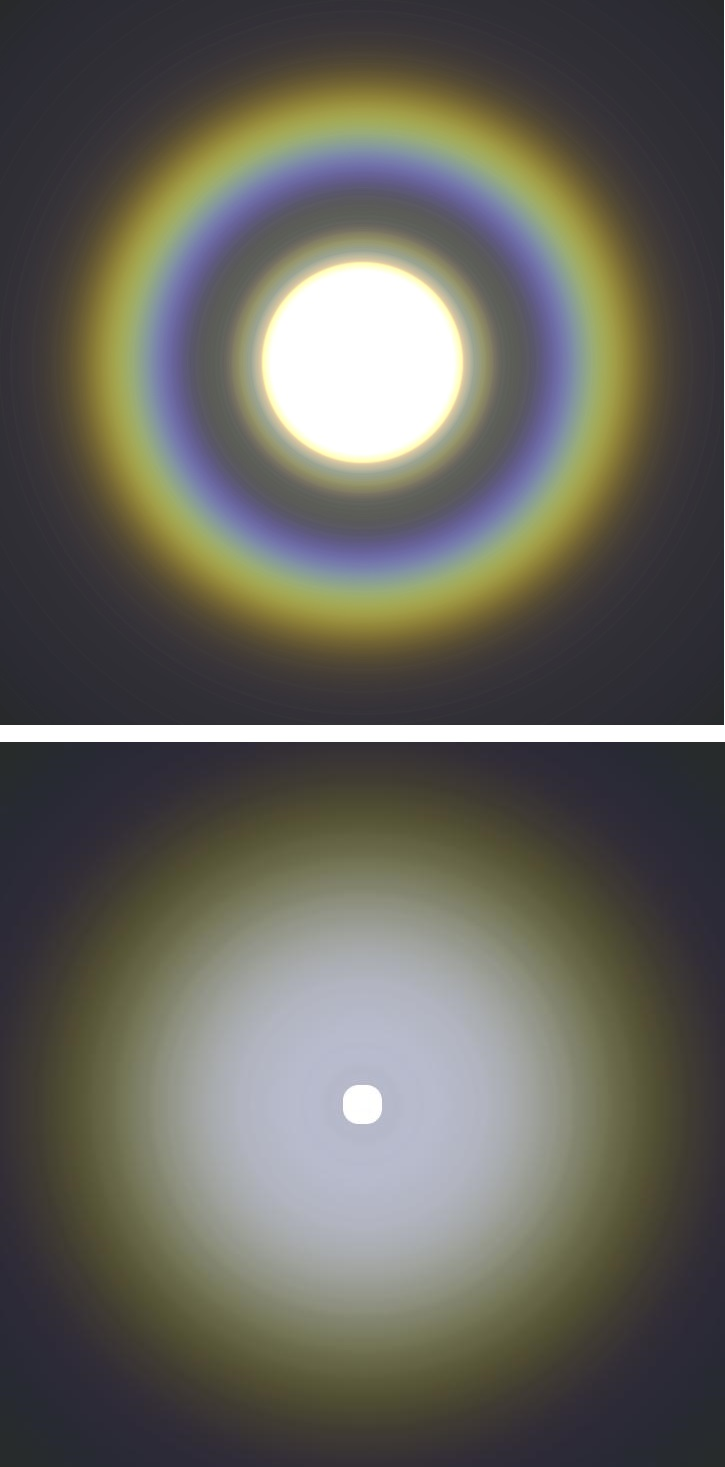
\includegraphics[height=\resLen]{slab/color4x_all.jpg}
        \\
        \textbf{(a) Phase function} & \textbf{(b) Thin-slab rendering}
    \end{tabular}
    \caption{\label{fig:multiwave1}
        \textbf{Multi-spectral results:} (a) visualizations of phase functions; (b) corresponding multi-spectral renderings of a thin slab lit by a small area light from behind.
        Results on the top are generated using a cluster of 100 particles with radii 500nm.
        Results on the bottom are obtained using a conventional single-particle setting.
        We used identical particle counts per differential volume for both configurations.
    }
\end{figure}
